\chapter {Ograničavajući volumeni (eng. Bounding volumes)}

Ograničavajući volumeni su jednostavni volumeni kojima ograničavamo objekte da bi olakšali i ubrzali detekciju sudara. Ponekad, u praksi, imamo objekte i poligone između kojih je teško detektirati sudar. U tom slučaju, primitivi kojima ograničimo objekt, mogu nam znatno olakšati detektiranje sudara \cite{1}. Umjesto da provjeravamo sudar između objekata, mi provjeravamo sudar između volumena koji ograničavaju objekt. Prednost toga je, kao što je već rečeno, znatno lakše detektiranje sudara, a mana je u tome što nikada ne možemo točno ograničiti objekt pa ćemo i ponekad detektirati sudar koji se nije dogodio.
\begin{figure}[!http]
	\begin{center}
		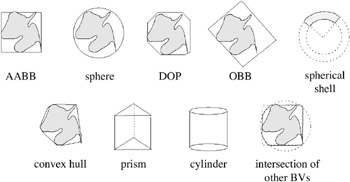
\includegraphics[height=6 cm, width = 6 cm, keepaspectratio = true]{bounding_volumes}
		\caption{Primjeri ograničavajućih volumena}
		\label{fig:1}
	\end{center}
\end{figure}

Kako je prikazano na slici \ref{fig:1} postoji puno ograničavajućih volumena\cite{1}. U ovom radu biti će objašnjen AABB tj. Axis Aligned Bounding Box. Razlog tomu je AABB stablo koje se koristilo kasnije kao Bouning Volume Hierarchy, no o tome će biti riječi kasnije.

\section{AABB - Axis Aligned Bounding Box}

Kao što i samo ime govori, AABB je ograničavajući kvadrat koji je poravnat sa koordinatnim osima. Ovo je i ujedno najjednostavniji, ali i najbrži ograničavajući volumen\cite{1}.U 3D geometriji, kvadrat ima 6 stranica, a u 2D geometriji to je pravokutnik (sa 2 strane) \cite{1}. 
\begin{figure}[!http]
	\begin{center}
		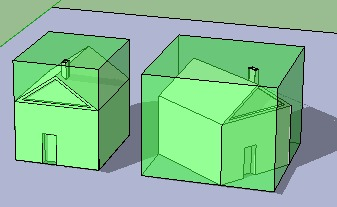
\includegraphics[height = 8 cm, width = 8 cm, keepaspectratio = true]{aabb}
		\caption{Axis Aligned Bounding Box prikazan zelenom bojom}
		\label{fig:2}
	\end{center}
\end{figure}

S obzirom da je AABB najjednostavniji oblik volumena, on nije uvijek točan. Ograničeni smo na korištenje pravokutnika pa iz toga slijedi da nećemo moći ograničiti objekt na onaj način na koji bismo željeli tj. postojati će neki "offset". U tom slučaju može se dogoditi da detektiramo sudar između objekata iako se on nije dogodio kao što je prikazano na slici.

\begin{figure}[!http]
	\begin{center}
		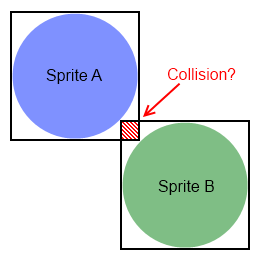
\includegraphics[height = 8 cm, width = 8 cm, keepaspectratio = true]{AABB_collision}
		\caption{Detektirani sudar između AABB-a koji se nije dogodio između objekata}
		\label{fig:2-1}
	\end{center}
\end{figure}

AABB u kodu možemo prikazati na nekoliko načina. Postoje 3 različite reprezentacije\cite{1} te ćemo u nastavku proći kroz sve, te pobliže opisati opisati onu koja se koristila u ovome radu.

\subsection{Reprezentacije AABB-a}\label{sec::AABB_representation}

Prva i ona najčešća reprezentacija je reprezentacija koja koristi minimalnu i maksimalnu točku objekta.
Ukratko, pronađemo minimalnu i maksimalnu točku x,y i z koordinate te od tih točki napravimo kvadrat ako smo u 3D geometriji, tj. pravokutnik ako smo u 2D\cite{1}.

\begin{lstlisting}[style = {myC++},label ={code:1}, caption = {Struktura AABB-a koji koristi min i max točke}]
struct AABB{
	float min[3];
	float max[3];
}

\end{lstlisting}
\begin{figure}[!http]
 	\begin{center}
 		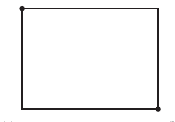
\includegraphics[height = 5 cm, width = 5 cm, keepaspectratio = true]{AABB_min-max}
 		\caption{AABB min-max reprezentacija u 2D geometriji}
 		\label{fig:3}
 	\end{center}
 \end{figure}
\newpage
Detektiranje sudara za ovu reprezentaciju je trivijalna. Provjerava se je li jedna koordinata minimalne točke jednog AABB-a veća od maksimalne koordinate točke drugog AABB-a ili obrnuto. Ukoliko to nije slučaj u sve 3 dimenzije, događa se sudar\cite{1}.

\begin{lstlisting}[style = {myC++},label={code:2}, caption = {Provjeravanje sudara za min-max reprezentaciju AABB-a\cite{1}}]
bool Collision(AABB a, AABB b)
{
	if (a.max[0] < b.min[0] || a.min[0] > b.max[0]) return 0;
	if (a.max[1] < b.min[1] || a.min[1] > b.max[1]) return 0;
	if (a.max[2] < b.min[2] || a.min[2] > b.max[2]) return 0;
	return 1;
}

\end{lstlisting}

Druga reprezentacija je korištenje minimalne točke i dijametra tj. udaljenosti do ostalih vrhova. Određivanje ovakvog volumena malo je kompliciranije nego u prethodnom slučaju upravo zbog dijametra koji moramo odrediti da bi ograničili objekt.

\begin{lstlisting}[style={myC++},label={code:3}, caption = {Struktura AABB-a koji koristi min točku i dijametar}]
struct AABB{
	float min[3];
	float dx,dy,dz; //udaljenost od minimalne tocke
}
\end{lstlisting}
 
 \begin{figure}[!http]
 	\begin{center}
 		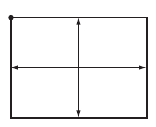
\includegraphics[height = 5 cm, width = 5 cm, keepaspectratio = true]{AABB_min-diametar}
 		\caption{AABB min-dijametar reprezentacija u 2D geometriji}
 		\label{fig:4}
 	\end{center}
 \end{figure}


Detekcija sudara je za ovu reprezentaciju također malo kompliciranija nego u prethodnom slučaju i najmanje je "privlačna" od sve 3 reprezentacije \cite{1}.


\begin{lstlisting}[style = {myC++},label={code:4}, caption = {Provjeravanje sudara za min-width reprezentaciju AABB-a\cite{1}}]
bool Collision(AABB a, AABB b)
{
	float t;
	if ((t = a.min[0]- b.min[0]) > b.d[0] || -t > a.d[0]) return 0;
	if ((t = a.min[1]- b.min[1]) > b.d[1] || -t > a.d[1]) return 0;
	if ((t = a.min[2]- b.min[2]) > b.d[2] || -t > a.d[2]) return 0;
	return 1;
}
\end{lstlisting}

Posljednja reprezentacija, i ona koju smo koristili u radu, jest centar i radijus. Odredimo središnju točku našeg AABB-a i radijus u svim osima kojima izradimo AABB. Ova reprezentacija je najučinkovitija u terminima uštede memorije\cite{1}. 

\begin{lstlisting}[style = {myC++},label={code:5}, caption = {Struktura AABB-a koji koristi centar i radijus}]
struct AABB{
float center[3];
float rad[3]; //radijus
}
\end{lstlisting}

 \begin{figure}[!http]
 	\begin{center}
 		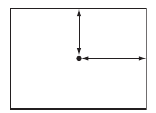
\includegraphics[height = 5 cm, width = 5 cm, keepaspectratio = true]{AABB_center-rad}
 		\caption{AABB centar-radijus reprezentacija u 2D geometriji}
 		\label{fig:5}
 	\end{center}
 \end{figure}
 \newpage
 Detektiranje sudara, za ovu reprezentaciju, je trivijalno. Za svaku dimenziju provjeravamo odnose centara i radijusa u svakoj dimenziji.
 
\begin{lstlisting}[style={myC++},label={code:6},caption={Provjeravanje sudara za centar-radijus reprezentaciju AABB-a\cite{1}}]
bool Collision(AABB a, AABB b)
{
	 if (Abs(a.c[0] - b.c[0]) > (a.r[0] + b.r[0])) return 0;
	 if (Abs(a.c[1] - b.c[1]) > (a.r[1] + b.r[1])) return 0;
	 if (Abs(a.c[2] - b.c[2]) > (a.r[2] + b.r[2])) return 0;
	 return 1;
}
\end{lstlisting}

Razlog biranja ove reprezentacije AABB-a leži u tome što smo odabrali kuglice kao objekte između kojih ćemo provjeravati sudar. S obzirom da je sfera, kao objekta, definirana centralnom točkom i radijusom, ova reprezentacija je odabrana kao najpogodnija.

\section{Kuglice}\label{sec:balls}

Kao što je već ranije spomenuto, objekti koji će se koristiti za detektiranje sudara u prostoru su kuglice tj. sfere. Kuglice su odabrane iz razloga što se vrlo jednostavno može odrediti fizikalna reakcija na sudar i što se na njih mogu lijepo primijeniti vanjske sile kao gravitacija i slično. Samim korištenjem kuglica i prijašnjim odabirom AABB-a kao ograničavajućih volumena javljaju se pojedini problemi.

Problem u ovome slučaju je već spomenut. Naime, kako je to i prikazano na slici \ref{fig:2-1}, AABB ograniči prostor koji sfera ne pokriva tj. prostor koji je izvan sfere. To se može objasniti vrlo jednostavnom matematikom. Ako prikažemo stranicu kvadrata kao:
\begin{equation}
a = 2r \label{eq:stranica}
\end{equation}
gdje nam je r radijus sfere tj. kuglice. Dalje, dijagonala kvadrata iznosi:
\begin{equation}
diag = a  \sqrt{2} \label{eq:dijagonala}
\end{equation}
Može se zaključiti da je udaljenost od sjecišta dijagonala tj. centra kvadrata veća od radijusa sfere za $\sqrt{2}$. Što je veća sfera to je pogreška u ograničavajućem volumenu također veća. Zbog toga će se sigurno događati da ćemo otkrivati sudare i onda, kada se oni ne događaju, a pri vrlo velikim sferama to može stvarati puno nelogičnosti i čudnih fizikalnih reakcija na sudar.Kada su sfere vrlo malog radijusa, ta pogreška se u principu i ne primjeti, ali je ipak prisutna.

Ovome problemu uskače se na vrlo dobar način. Kako je prikazano na slici \ref{fig:1}, sfera sama po sebi može biti ograničavajući volumen \cite{1}. To proizlazi iz činjenice da se na vrlo jednostavan i elegantan način može detektirati sudar između 2 sfere. 

\begin{lstlisting}[style = {myC++},label={code:6-1}, caption = {Detekcija sudara između 2 sfere\cite{1}}]
bool SphereCollision(Sphere a, Sphere b)
{
// Calculate squared distance between centers
Vector d = a.c - b.c;
float dist2 = Dot(d, d);
// Spheres intersect if squared distance is less than squared sum of radii
float radiusSum = a.r + b.r;
return dist2 <= radiusSum * radiusSum;
}
\end{lstlisting}
U stvarnom kodu, implementacija ove funkcije izgleda drugačije nego što je opisana ovdje i u literaturi\cite{1}, ali u principu algoritam i pristup su jednaki.
\newpage
\subsection{Implementacija klase za kuglice}

Implementacija klase za kuglice u principu je jednostavna. Prikazana je sljedećim kodom:

\begin{lstlisting}[style = {myC++},label={code:7}, caption = {Implementacija klase za kuglice}]
public:
	Vector3D vecDir;
	AABB_box bBox;
	
	Ball() = default;
	Ball(const Point center, const float r, const float vecX, const float vecY,
		const float vecZ, const float m, const uint i);
	Ball(const float x, const float y, const float z, const float r,
		const float vecX, const float vecY, const float vecZ, const float m,
		const uint i);	
	void drawSphere();;
	void updatePosition(const float dt);
	bool collision(Ball &collider);
	template <typename T> bool collision(T &collider) {
		return isOverlap(this->bBox, collider.bBox);
	}
	void resolveCollision(Ball &collider);
	void resolveCollision(Wall &wall);
	Point &getCenter() { return this->center; }
	const float &x() const { return this->center.x; }
	const float &y() const { return this->center.y; }
	const float &z() const { return this->center.z; }
	const float &rad() const { return this->r; }
	const float &getMass() const { return this->mass; }
	const uint &getI() const { return this->i; }
private:
	Point center;
	float r;
	float mass;
	uint i;
};

\end{lstlisting}

Da se primijetiti da se u samoj deklaraciji klase uglavnom nalaze konstruktori i get metode za dobivanje privatnih varijabli. \emph{Get} i \emph{template} metode su definirane u samoj deklaraciji klase zbog svoje jednostavnosti i veće brzine pristupanja.

U privatnim varijablama klase definirali smo najvažnije informacije o kuglici, a to su:

\begin{itemize}
	\item $Center$ - točka centra za svaku kuglicu
	\item $r$ - radijus sfere
	\item $mass$ - masa sfere koja se kasnije koristi za količinu gibanja
	\item $i$ - pozicija kuglice u listi kojom se osigurava da kuglica ne provjerava sudar sa samom sobom 

\end{itemize}

U javnim varijablama odredili smo:
\begin{itemize}
	\item $bBox$ - odgovarajući AABB koji je opisan prethodno
	\newline
	U ovom slučaju $bBox$ dobiva vrijednosti radijusa i centra od sfere kroz konstruktor
	\item $vecDir$ - vektor definiran u klasi \emph{Vector3D} koja sadrži osnovne operacije nad vektorima (skalarni produkt, oduzimanje, normaliziranje i sl.)
	\newline
	Ovaj objekt nam omogućava kretanje kuglice i olakšava izračunavanje sudara od zida i druge kuglice. Implementacija same klase biti će pokazana u kasnijim poglavljima.
	
\end{itemize}

Metode koje su definirane, u konačnosti govore same za sebe:
\begin{itemize}
	\item $collision$ - detektira sudar kuglice ovisno o tipu s kojim se sudara.\newline
	Ukoliko se događa sudar sa drugom kuglicom, sudar se detektira na ranije opisani način. Sudar sa zidom i bilo kojim drugim objektom se detektira preko pridodanih AABB-a.
	\item $resolveCollision$ - u metodama ovog imena definiramo fizikalnu reakciju kuglice na sudar. Ovisno o objektu s kojim se kuglica sudara, tako se i poziva određena $resolveCollision$ funkcija
	\item $drawSphere$ - funkcija za crtanje kuglica
	\newline
	Kuglice u prvom trenutku crtamo sa \emph{glutSolidSphere} i pomoću \emph{glTranslatef} ih pomičemo po prostoru. Kasnije, pri korištenju Opengl 3.3 kuglice će se crtati na drugačiji način.
	\item $updatePosition$ - metoda kojom definiramo kretanje kuglica po prostoru uz pridodanu gravitaciju. \newline
	Detaljnija implementacija će biti kasnije objašnjena
\end{itemize}

U glavnom programu kuglice smo spremali u  \emph{std::vector}. Na taj način smo jednostavno iterativnim prolaženjem kroz listu iscrtavali kuglice, detektirali sudar između kuglica i zidova i u konačnosti pomicali kuglice po prostoru.
 